\documentclass{abrice}

\title{Comp 549: Assignment 3}
\author{Anthony Brice}

\begin{document}
\maketitle

\section{Part 1}

\subsection{Punching Data on Computer Cards}

\marginnote{Anna Bieszczad has always maintained that in college she turned her
  homework in with punch cards. I've always wondered if Western schools still
  used punch cards by that time.} That hardly seems like a desirable way to
interact with the computer. They really required a machine of that size to
manufacture punch cards?

\subsection{1963 Timesharing: A Solution to Computer Bottlenecks}

While I agree with Kay's conclusion discussed below that the ``desires for
flexibility, resolution, and response'' naturally lead to ``the possibility of
giving each person his own powerful machine'' as opposed to timeshared
computing, I would neither dismiss the advancements displayed in this video as
an evolutionary dead-end. The methodologies pioneered here are ones fundamental
to cloud-computing platforms like Amazon Web Services, and the idea of putting
hardware to use while it would remain otherwise idle powers projects such as
Folding@home.

What I find most surprising is that this might be the first time we've seen a
REPL in any of our videos. It seems natural that such an idea might grow out of
a need to have many terminals interacting with a single machine, but I had never
thought of it like that before.

\subsection{Xerox PARC Demo for Apple (1979)}

If you look closely at the start of the video, it looks like the top-most window
might be displaying a Miller column browser.

All in all it lacks a common menu bar and window decorations, but it doesn't
seem that different from Apple's soon-to-come offering. \marginnote{EVEN THE
  FRENCH!}

\section{Part 2}

\subsection{Personal Dynamic Media, Kay and Goldberg}

What I take away most from the essay is Kay's emphasis on user-centered
design. Early on he makes clear that in designing the dynabook they ``focus[ed]
on children [their] user community.'' This novel approach seems to have worked
wonders keeping Kay and his team honest about their work. His assertion that
when ``they are doing \emph{real} things rather than playing with toys or
working out `assigned' problems \ldots\ their attention spans are measures in
hours rather than minutes [emphasis in the original]'' aligns with my own
experience tutoring young children with MIT's Scratch educational programming
language.

In addition to captivating children, user-centered design led Kay and his team
to many breakthroughs we take for granted today. They envision computers as not
just devices for calculating difficult math programs, but as tools for music
composition, graphic design, and animation---all on a display ``\emph{not}\,
\ldots\ \emph{worse} than paper in any important way [emphasis in the
original]'' with fonts ``of publishing quality.''\marginnote{A man after my own
  heart.}

Indeed, I think the design philosophy led them to a vital realization we had yet
to come across in our reading: that a computer's ``ability to simulate the
details of any descriptive model means that the computer, viewed as a medium
itself, can be \emph{all other media} if the embedding and viewing methods are
sufficiently well provided,'' or that computers are a ``metamedium'' as he goes
on to call them. In hindsight the idea seems to follow naturally from the
concept of computers as universal Turing machines, where implementing all of
untyped lambda calculus means a computer can compute anything
computable\marginnote{This concept seems lost on our Congress. They think they
  can legislate the market into selling computers with no ability to encrypt
  their contents. Doing so would mean they no longer sell computers.}, but
nowhere have we seen the idea expressed so clearly and succinctly.

Kay goes on to argue that this new metamedium can combine ``the flexibility and
generality'' of ``paper and clay\, \ldots\ with tools which have the power'' of
``cars and television sets,'' but I would argue that here his team's approach of
user-centered design before all else hinders their progress towards that goal.
For software tools to be truly useful they need to be modular. They not only
need a great interface from which the user interacts but also a common interface
in which the tools interact with each other, and I do not think we see that in
his examples of tools designed for the Dynabook. These programs are monolithic,
drawing from features implemented in the Smalltalk language but not from each
other.

\subsection{User Interface: A Personal View, Kay}

From this essay I most took away the psychological underpinnings of Kay's
user-centered design. Kay expresses his approach to design as ``Doing with
Images makes Symbols,'' where \emph{doing} refers to manipulation, \emph{images}
to the iconic, and \emph{symbols} to the abstract.

I find this to be a wonderful metaphor and the practical design of a user
interface he cites gels perfectly with it. Particularly I like how this leads
him to the conclusion ``that everything should be made modeless,''
\marginnote{One can infer that Kay had no love for \texttt{vim}.} a central
design tenet still espoused in Apple's human interface guidelines. In fact,
features like iOS's Home button, which ensures ``the user could always get to
the next thing desired without any backing out,'' can be traced directly back
it.

As in the previous essay, I think Kay lets user-centered design to some extent
cloud his judgment. He notes that ``personal computing has concentrated mostly''
on the fact that ``we communicate with our selves [and] our tools,'' but
neglects or forgets that it also must concentrate on the face that our tools
must communicate with our tools.

\section{Part 3}

\emph{Create a prototype of an interactive system for the following scenario: A
  local theater wants an app that will allow users to see what is playing at the
  theater over a range of dates that may span up to 3 months. Users can select
  a particular show and then view availability of tickets and purchase tickets
  by using their credit cards.  The app should also provide access to other
  information such as location and business hours, and also have links to its
  facebook and twitter.}

\begin{figure*}
  \caption{The app's home screen, information screen, and particular show
    screen.}
  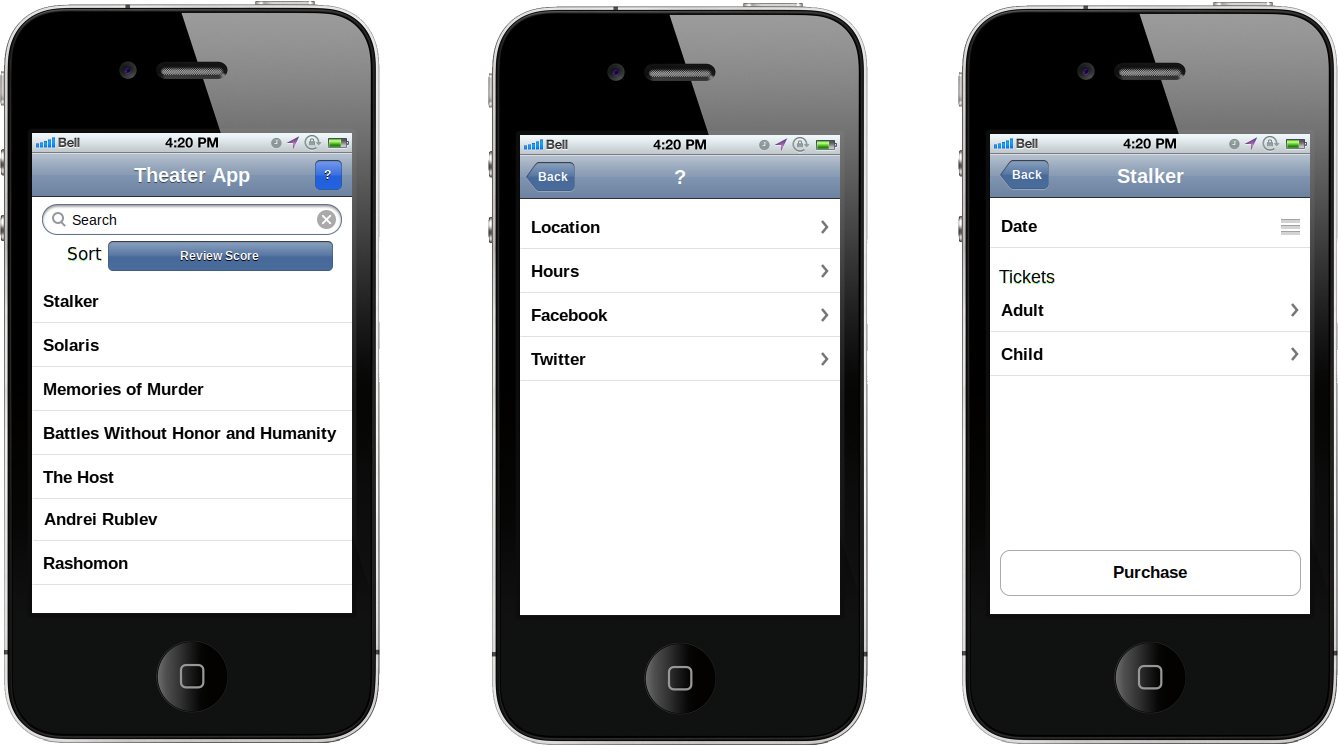
\includegraphics[height=8cm]{phones}
\end{figure*}

\noindent
The interactive system describes a few tasks the user should be able to
perform. The first of these and surely the most common is that of selecting a
particular show, so it is readily available from the home screen. I chose menu
selection for the task mainly for its ease of use---the home screen should be
intuitive; we don't want to scare anyone away---and because it seems natural
that a state change of the interface would follow selecting a particular show.

From there a few subtasks follow, and I bundled those into a form fill-in. The
user selects a date, selects the number of adult and/or child tickets, and
purchases his or her tickets. The heavy use of data entry here necessitated a
style that would make it as simple as possible. That the style consumes screen
space is mitigated by the fact that we don't have a whole lot to show the user
here.

The last task the system describes is the access of information such as
location, hours, and social media presence. Again these are presented as menu
selection. For the latter the style is necessary since either a web browser or
the social media provider's app would launch upon selection.

\end{document}

%%% Local Variables:
%%% mode: latex
%%% TeX-master: t
%%% End:

%  LocalWords:  metamedium dynabook subtasks
